\documentclass{report}

% Language setting
\usepackage[main=portuguese, english]{babel}
\usepackage{csquotes}

% Set page size and margins
\usepackage[a4paper,top=2cm,bottom=2cm,left=3cm,right=3cm,marginparwidth=1.5cm]{geometry}

% Useful packages
\usepackage{ulem}
\usepackage{parskip}
\usepackage{indentfirst}
\usepackage{setspace}
\usepackage{amsmath}
\usepackage{array}

\usepackage{graphicx}
\usepackage{xcolor}
\usepackage{colortbl}
\usepackage{subfigure}
\usepackage{titlesec}
\usepackage[colorlinks=false, allbordercolors={0 0 0}, pdfborderstyle={/S/U/W 0.25}]{hyperref}
\usepackage[hypcap=true]{caption}
\usepackage{enumitem}
\usepackage{soul}

\usepackage[backend=biber,]{biblatex}
\addbibresource{reference.bib}

% Set section numbering from 1.1
\renewcommand{\thesection}{\arabic{section}.1}

\let\oldsection\section
\renewcommand\section{\clearpage\oldsection}

% Change section formatting
\titleformat{\section}
  {\fontsize{12}{15}\selectfont\bfseries}{\thesection}{1em}{}

% Configure indentations
\setlength{\parindent}{1.5cm}

\begin{document}

    \begin{titlepage}
        \centering
        
        \LARGE {Universidade Federal do Rio Grande do Sul \\ Instituto de Informática}
    
        \begin{figure}[h!]
        \centering
        \subfigure
        {
\includegraphics[width=0.35\linewidth]{images/logos/UFRGS.png}}
        \hspace{1cm}
        \subfigure
        {
\includegraphics[width=0.35\linewidth]{images/logos/INF.png}}
        \end{figure}
    
        \LARGE {INF01017 \\ Aprendizado de Máquina}
        
        \vfill
        {\noindent\hrulefill \\
        \bfseries \Huge{Trabalho Prático Final – Etapa 1} \\ \LARGE{Predição de Consumo de Combustível} \\
        \noindent\hrulefill}
        
        \vfill
        {\LARGE Luís Filipe Martini Gastmann (00276150) \\ Pedro Lubaszewski Lima (00341810) \\ Vinícius Boff Alves (00335551) \\~\\ Turma U}
    
        \vfill
        {\LARGE 9 de novembro de 2024}
        
    \end{titlepage}

        \renewcommand{\contentsname}{Sumário}
        \tableofcontents
        \clearpage
        \addtocontents{toc}{\protect\thispagestyle{empty}}

\section{Definição do Problema e Coleta de Dados}

O objetivo deste trabalho é prever o consumo médio de combustível de um carro através de algumas das suas características e origens de fabricação.
Alguns atributos das instâncias são a marca, a quantidade de cilíndros, o porte do veículo etc.

O conjunto de dados utilizado para desenvolver este trabalho foi obtido da seguinte página do Kaggle:
\href{https://www.kaggle.com/datasets/arslaan5/explore-car-performance-fuel-efficiency-data}{Explore Car Performance: Fuel Efficiency Data}.
Essa tarefa contará com diversas técnicas de preparação dos dados para posteriormente iniciar a seleção e
avaliação de modelos para essa tarefa.

\section{Análise Exploratória e Pré-processamento dos Dados}

\subsection{Análise Exploratória dos Dados}

Este \textit{dataset} possui 550 instâncias, com 11 atributos preditores e 1 atributo alvo. Esse último torna a tarefa dos modelos em regressão,
visto que o objetivo aqui é prever o consumo médio de combustível de carros. No conjunto de dados, esse atributo predito se chama \textit{combination mpg}.

Dos atributos preditores, observa-se que há 5 atributos numéricos (\textit{city mpg}, \textit{cylinders}, \textit{displacement}, \textit{highway mpg} e \textit{year}).
Além deles, os 6 atributos restantes são categóricos: \textit{class}, \textit{drive}, \textit{fuel type}, \textit{make}, \textit{model} e \textit{transmission}.
Com isso em mente, criou-se alguns gráficos para analisar correlações e distribuições dos dados. A seguir, o \textit{violin plot}
do atributo alvo pelo número de veículos:

\begin{figure}[h!]
  \centering
  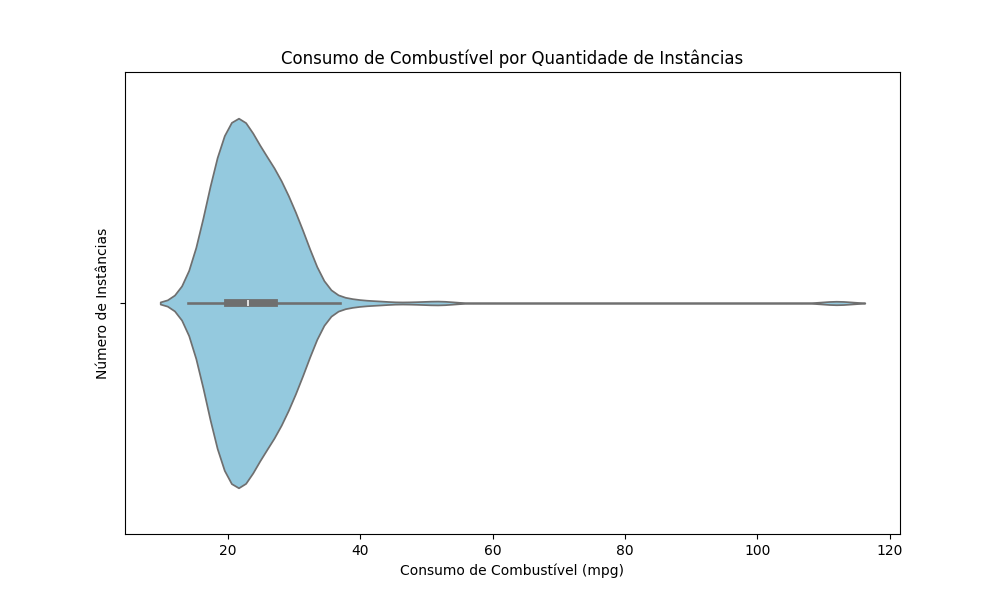
\includegraphics[width=.85\linewidth]{images/plots/violin_plots/pure_combination_mpg.png}
  \caption{\label{img:combination_dist} \textit{Violin Plot} de Consumo Médio}
\end{figure}

Nesse ponto, já se observa que há instâncias problemáticas, claramente \textit{outliers} que devem ser removidas do conjunto de dados. Ademais, a maior concentração dos veículos
apresenta consumo médio entre 15 e 30mpg, algo que pode guiar bastante os modelos. Após isso, analisou-se o atributo de classes de veículos para ter uma ideia da sua distribuição
em um gráfico de setores.

\begin{figure}[h!]
  \centering
  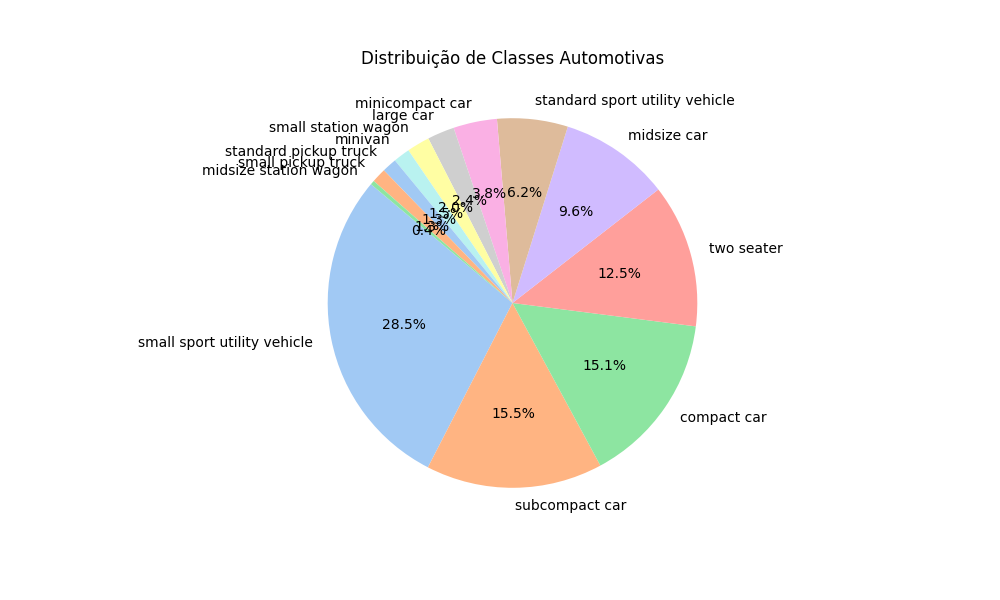
\includegraphics[width=.85\linewidth]{images/plots/pie_charts/pure_car_classes.png}
  \caption{\label{img:classes_dist} Distribuição de Classes de Veículos}
\end{figure}

Com ele, é perceptível que talvez seja necessário agrupar as classes de veículos e outros atributos que contenham classes com muito poucos representantes, como \textit{midsize station wagon},
por exemplo, em uma classe geral chamada \textit{others}. Porém, isso será melhor analisado, se necessário, na segunda etapa do trabalho. No entanto, algo que é necessário é a codificação dos
atributos categóricos em numéricos para padronizar a entrada numérica dos modelos.

Por fim, analisou-se a Correlação de Pearson entre os atributos numéricos através do \textit{heatmap} abaixo:

\begin{figure}[h!]
  \centering
  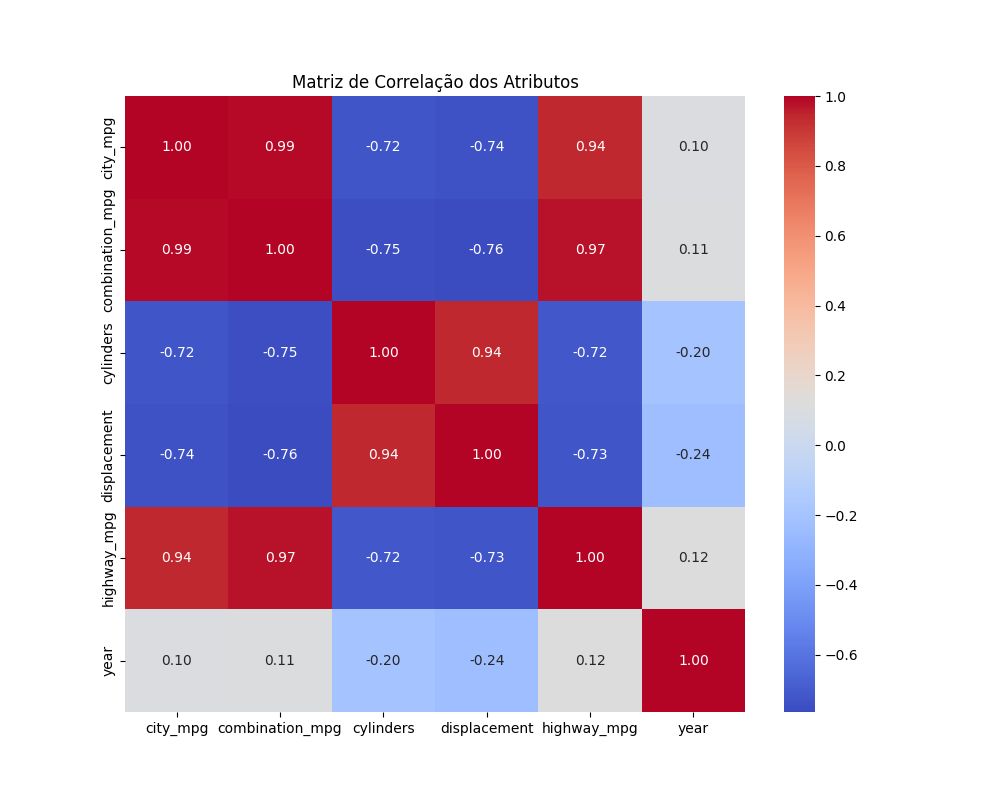
\includegraphics[width=.85\linewidth]{images/plots/heatmaps/numeric_atributes_correlation.png}
  \caption{\label{img:num_heatmat} \textit{Heatmap} de Correlações entre Atributos Numéricos}
\end{figure}

Olhando para o gráfico acima, percebe-se que há diversos atributos preditores que apresentam alto nível de correlação com a saída \textit{combination mpg} e entre si. Ambos os atributos
\textit{highway mpg} e \textit{city mpg} serão descartados do \textit{dataset} por terem alta correlação entre si e com o valor da saída do modelo, facilitando demais a tarefa dos modelos.
Além disso, \textit{displacement} ou (exclusivo) \textit{cylinders} será excluído do conjunto de dados por terem alta correlação entre si.

Isto não foi ilustrado pelos gráficos, porém os dados numéricos apresentam diversas escalas diferentes, exigindo técnicas de normalização após a separação de conjuntos de treinamento/validação
e de testes.

\subsection{Pré-processamento dos Dados}

Como já discutido na seção acima e analisando alguns trabalhos realizados com esse conjunto de dados, esses sendo de Lunovian \cite{Lunovian}, da Ayşe \cite{Ayşe} e do Priyanshu \cite{Priyanshu},
implementou-se algumas estratégias de pré-processamento nos dados deste problema.

Primeiramente, realizou-se a remoção dos atributos discutidos anteriormentes. Esses sendo o \textit{highway mpg}, \textit{city mpg} e \textit{displacement}, visto que apresentam alto níveis de
correlação entre si e com o valor da saída do modelo. Após essa remoção, filtrou-se as instâncias com muitos atributos faltantes (em geral, carros elétricos que funcionam diferentemente dos carros
que funcionam com combustíveis fósseis).

Depois disso, foi realizada a limpeza de instâncias cujo atributo alvo representava um \textit{outlier} no gráfico de distribuição de consumo médio dos veículos. Essa estratégia é necessária para
evitar que os modelos sejam treinados com instâncias que não representam bem a grande a maioria dos veículos. Utilizou-se a medida padrão de 1.5 vezes o IQR para identificar \textit{outliers}.

Sobre a codificação dos atributos, o grupo utilizou a codificação padrão de categórico para numérico que é o \textit{one-hot encoding}. A justificativa para isso é que os atributos categóricos não
apresentam nenhuma ordem específica que justifique utilizar uma codificação em números inteiros. Além disso, em relação à normalização, baseado no trabalho do Jason Brownlee \cite{ColumnTransformer} e
do Matheus Vasconcelos \cite{PadronizarDados}, optou-se por utilizar a padronização por \textit{z-score}, visto que os dados aproximam uma distribuição normal. Tanto a codificação, quanto a normalização
foram aplicadas após a separação de conjuntos de treinamento/validação e de testes.

Um outro problema encontrado consiste na possibilidade de não ser visto algum modelo de carro (\textit{model}) no treinamento. Isso pode acontecer pois há uma quantidade muito grande de modelos diferentes,
alguns deles com poucas instâncias. Para solucionar esse problema, ``forçou-se" a haver pelo menos uma instância de cada modelo de veículo no conjunto de treinamento, antes de realizar a separação de
conjunto de dados para teste. Para realizar essa última separação, utilizou-se a função \texttt{train\_test\_split()} com um \texttt{test\_size} de 15\%. Essa ação corresponde à estragégia de \textit{holdout}
vista em aula para a primeira divisão dos dados.

\section{Abordagem, Algoritmos e Estratégias de Avaliação}

Seguindo as ideias discutidas nos ítens anteriores, este problema consiste em uma tarefa de regressão. Por conta disso, o grupo buscou no conteúdo programático da disciplina algoritmos para essa tarefa.
Com isso, separou-se os seguintes algoritmos de aprendizado para serem avaliados: \textbf{\textit{k-Nearest Neighbors}}, \textbf{\textit{Random Forest}}, \textbf{Regressão Linear}, \textbf{Redes Neurais}
e \textbf{SVM}. A escolha desses modelos também foi inspirada nos trabalhos de Neslihan Avsar \cite{LinearRegression}, de James McCaffrey \cite{Regression} e de isitapol2002 \cite{MultRegression}.

Definidos esses algoritmos e as estratégias de pré-processamento, definiu-se como estratégia de validação desses algoritmos o \textit{k-fold cross-validation}. Essa é a \textit{magnum opus} das estratégias
de validação de aprendizado supervisionado, então foi a adotada pelo grupo. O valor de \texttt{k = 13} foi definido experimentalmente. A justificativa mora na quantidade de instâncias que
sobraram para a validação após a separação de modelos de carros únicos para o treinamento e do conjunto de testes. O número final de elementos por \textit{fold} beira 18 instâncias (quantidade não muito grande,
porém proporcionalmente aceita para a quantidade total de instâncias do \textit{dataset}), gerando 13 medições de erro para cada modelo.

Em cada iteração do \textit{k-fold cross-validation}, realizou-se a normalização e a codificação dos atributos correspondentes através dos métodos adequados do \texttt{scikit learn}. Foi fixada um \texttt{random\_state = 42}
para padronizar os resultados dos testes. Os hiperparâmetros utilizados nesta etapa foram todos os padrões de cada modelo da biblioteca do \texttt{scikit learn}.

A métrica de avaliação utilizada foi o \textit{Mean Squared Error} (MSE). O grupo optou por sumarizar os resultados do \textit{spot-checking} com apenas esta métrica (descartando o \textit{Mean Absolute Error}) porque são métricas
de natureza muito similar, já foi realizada a limpeza de \textit{outliers} que poderiam prejudicar os resultados dessas medições e essa é uma métrica que apresenta convergência mais rápida (Nirajan Acharya \cite{MSEAndMAE}). Além
disso, foram feitas diversas representações dessa métrica para obter maior confiança nos resultados obtidos.

\section{\textit{Spot-checking} de Algoritmos}

\subsection{Revisitando os Dados após o Pré-processamento}

Com toda a metodologia explicada, voltar-se-á ao conjunto de dados pré-processados para realizar uma breve revisão dos dados de treinamento/validação. Primeiramente, após a remoção de \textit{outliers}, redução de dimensionalidade
e exclusão de instâncias de carros elétricos, gerou-se o seguinte gráfico de distribuição da saída a ser predita:

\begin{figure}[h!]
  \centering
  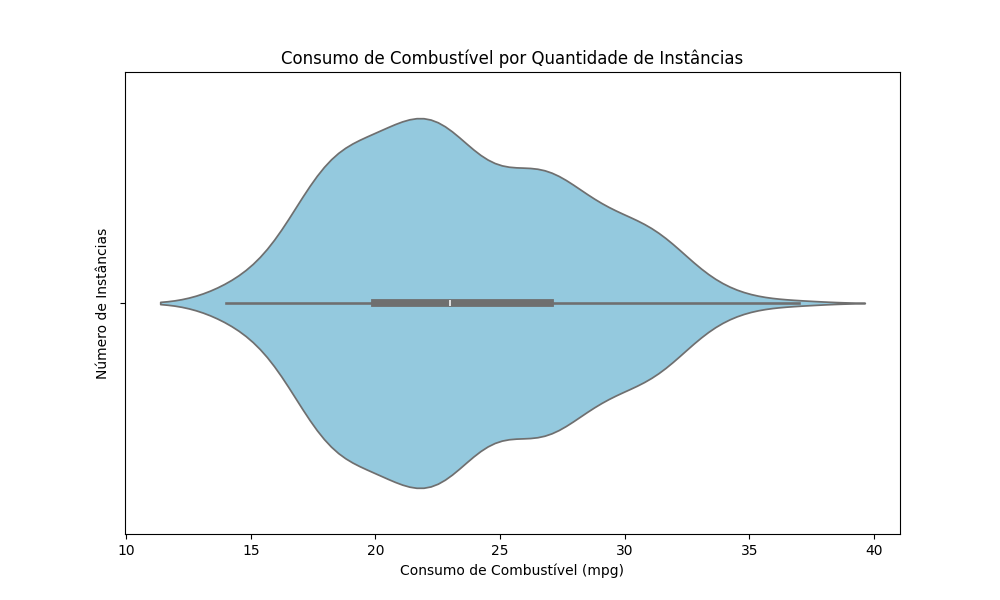
\includegraphics[width=.85\linewidth]{images/plots/violin_plots/no_outliers_combination_mpg.png}
  \caption{\label{img:pre_combination_dist} \textit{Violin Plot} de Consumo Médio Pré-processado}
\end{figure}

Agora observa-se que os dados quase se distribuem em formato de uma gaussiana. Além disso, continua observando-se a concentração de dados entre 15 e 30mpg de consumo médio. O gráfico de correlação também é refeito a seguir:

\begin{figure}[h!]
  \centering
  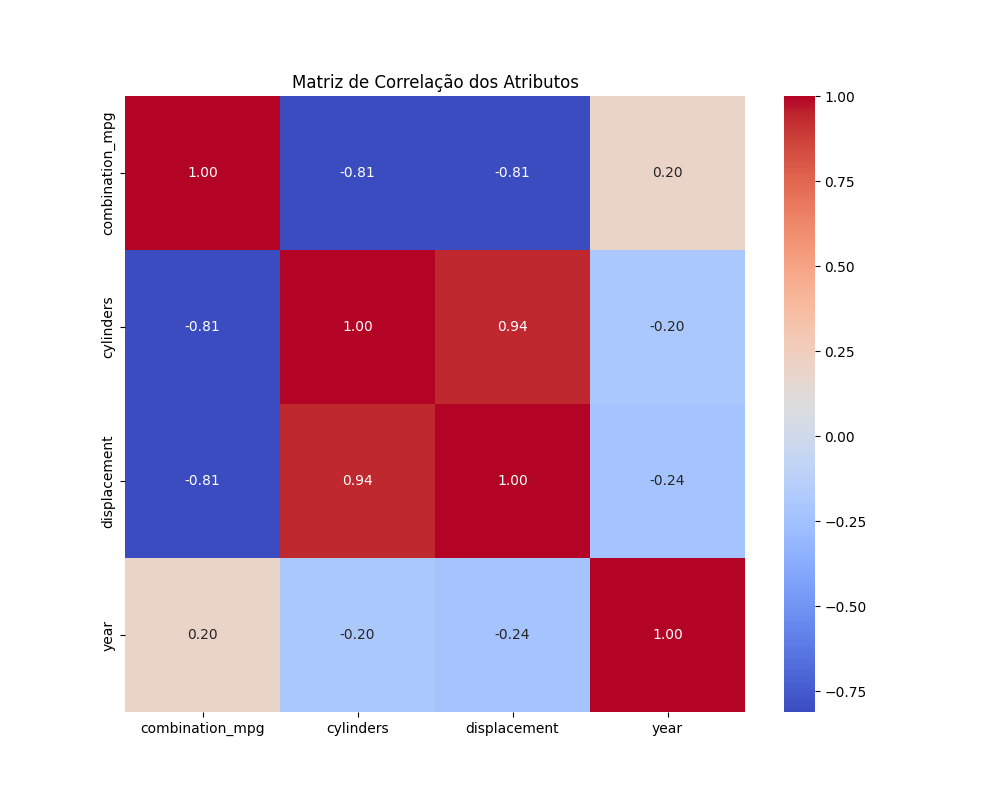
\includegraphics[width=.85\linewidth]{images/plots/heatmaps/no_outliers_numeric_atributes_correlation.png}
  \caption{\label{img:pre_num_heatmat} \textit{Heatmap} de Correlações entre Atributos Numéricos Pré-processados}
\end{figure}

Com a remoção dos atributos citados anteriormente, observa-se uma boa redução na correlação entre os atributos numéricos restantes. Algo que ajuda bastante a evitar a maldição da dimensionalidade.

\subsection{Sumarização dos Resultados}

Com esses dados revisitados, a seguir seguem os resultados obtidos pelos modelos:

\begin{table}[h!]
  \centering
  \begin{tabular}{| c | c | c |}
      \hline
      \rowcolor{lightgray}
      \textbf{Modelo} & \textbf{Média dos MSE} & \textbf{Desvio Padrão dos MSE} \\
      \hline
      kNN & 5,4293 & 2,3616 \\
      \hline
      \textit{Random Forest} & 1,9517 & 1,1847 \\
      \hline
      Regressão Linear & 1,6631 & 0,9758 \\
      \hline
      Redes Neurais & 1,8377 & 1,0418 \\
      \hline
      SVM & 3,3739 & 1,3368 \\
      \hline
  \end{tabular}
  \caption{\label{table:model_summary} Médias e Desvios Padrões dos MSE}
\end{table}

\begin{figure}[h!]
  \centering
  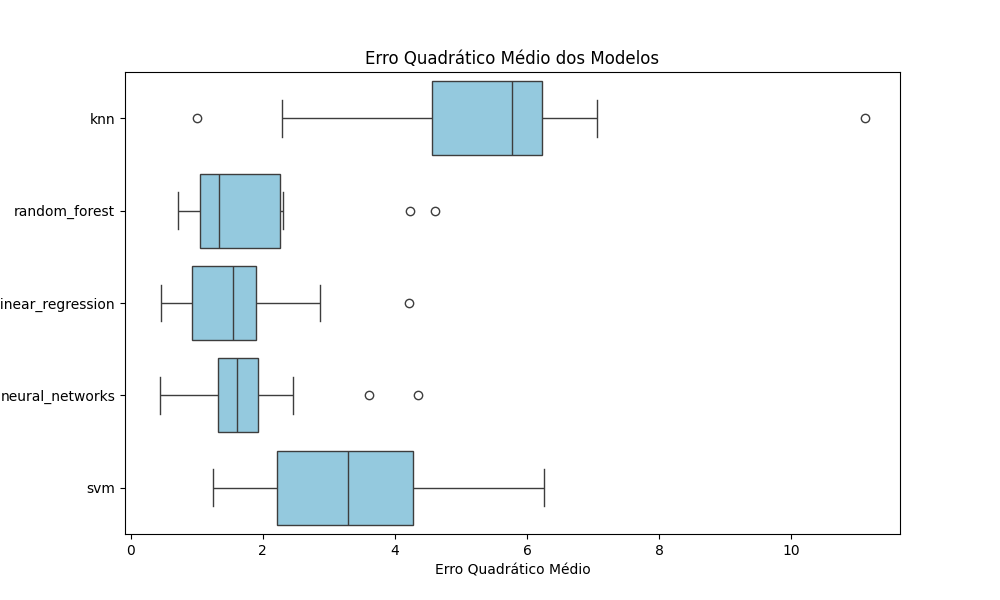
\includegraphics[width=.85\linewidth]{images/plots/box_plots/mse.png}
  \caption{\label{img:mse_boxplot} \textit{Box Plot} dos MSE}
\end{figure}

Por fim, com esses resultados, fica claro que os 3 modelos mais promissores foram a \textbf{\textit{Random Forest}}, a \textbf{Regressão Linear} e as \textbf{Redes Neurais}. Como nenhum atributo
foi otimizado, pode ser que os outros dois modelos se desempenhassem melhor, porém, com as configurações básicas de hiperparâmetros, esses foram os três mais promissores.

Dentre esses, é perceptível que os mais eficientes nesta tarefa foram o algoritmo de Regressão Linear e o modelo de Redes Neurais, visto que o viés da \textit{Random Forest} é mais elevado quando
comparado com esses últimos dois. Mesmo que a Regressão Linear apresente média e desvio padrão melhores do que as Redes Neurais, o \textit{box plot} acima mostra que o viés do erro das Redes Neurais
é mais concentrado, próximo de um valor estável. Por conta dessas razões, serão aprofundados as Florestas Aleatórias, o Regressor Linear e as Redes Neurais, com enfase nos últimos dois durante a
próxima etapa do projeto.

\clearpage
\printbibliography
\thispagestyle{empty}

\end{document}